\chapter{Diseño}

En esta sección se describirán las clases y todos los métodos que se han añadido y modificado durante el proceso de implementación.

\section{Diagrama de Clases}
Al compilar los archivos fuente y generar el proyecto, los archivos de configuración de CMake generan una serie de \emph{soluciones}. Hay soluciones que consisten únicamente en el archivo '\textit{main}', que representa el ejecutable al que llamamos por línea de órdenes desde la terminal. El resto de soluciones forman la propia API de OpenBabel, teniendo como clases principales 'OBMol', 'OBAtom', y 'OBBond', que permiten almacenar la información de una molécula, un átomo, o un enlace entre átomos respectivamente; y otras clases más orientadas a la conversión entre formatos como 'OBConversion' u 'OBFormat' (se explica más en detalle la estructura del proyecto OpenBabel y el proceso de compilación en el Anexo \ref{apend:manual}).

Para este trabajo, se ha necesitado modificar algunas clases de la API y añadir otras nuevas. En el siguiente Diagrama de clases (Figura \ref{fig:diagrama_clases}) se muestran tanto las clases que se han visto modificadas (en color anaranjado), las creadas desde cero (en color más verdoso) y las demás clases importantes que interactúan con las anteriores pero no se han visto alteradas (en amarillo).

\begin{landscape}

    \begin{figure}[]
        \centering
        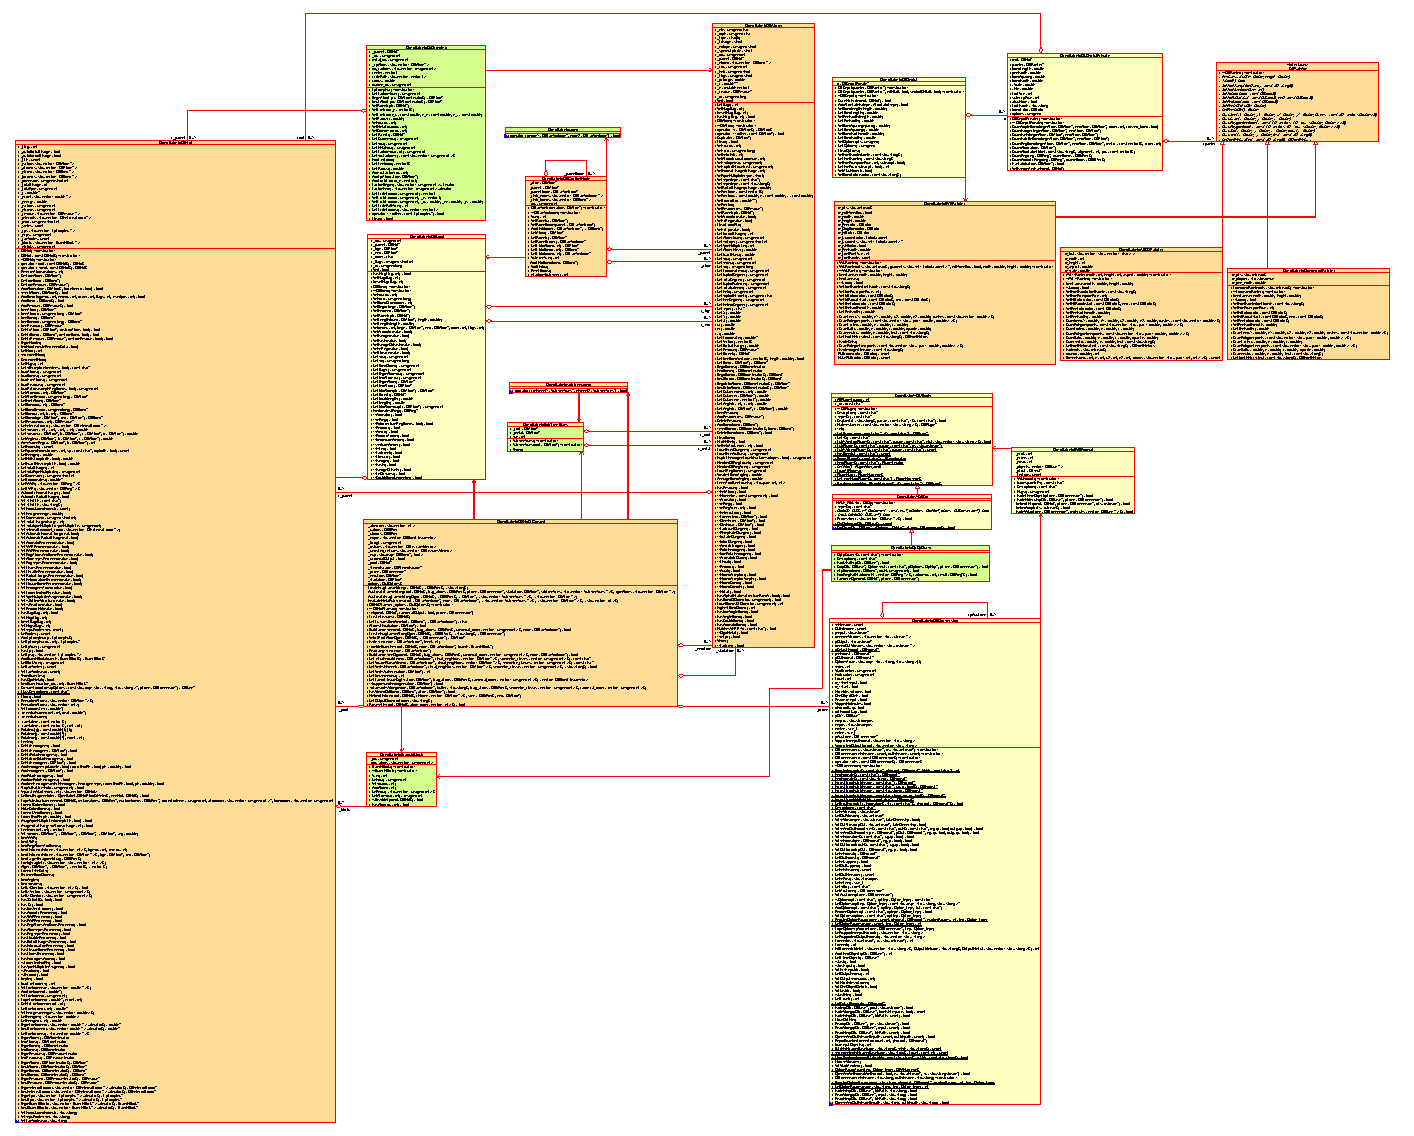
\includegraphics[scale=0.7]{imagenes/diseno/diagramaClasesHorizontal_cropped.pdf}
        \caption{Diagrama de clases}
        \label{fig:diagrama_clases}
    \end{figure}
\end{landscape}

% 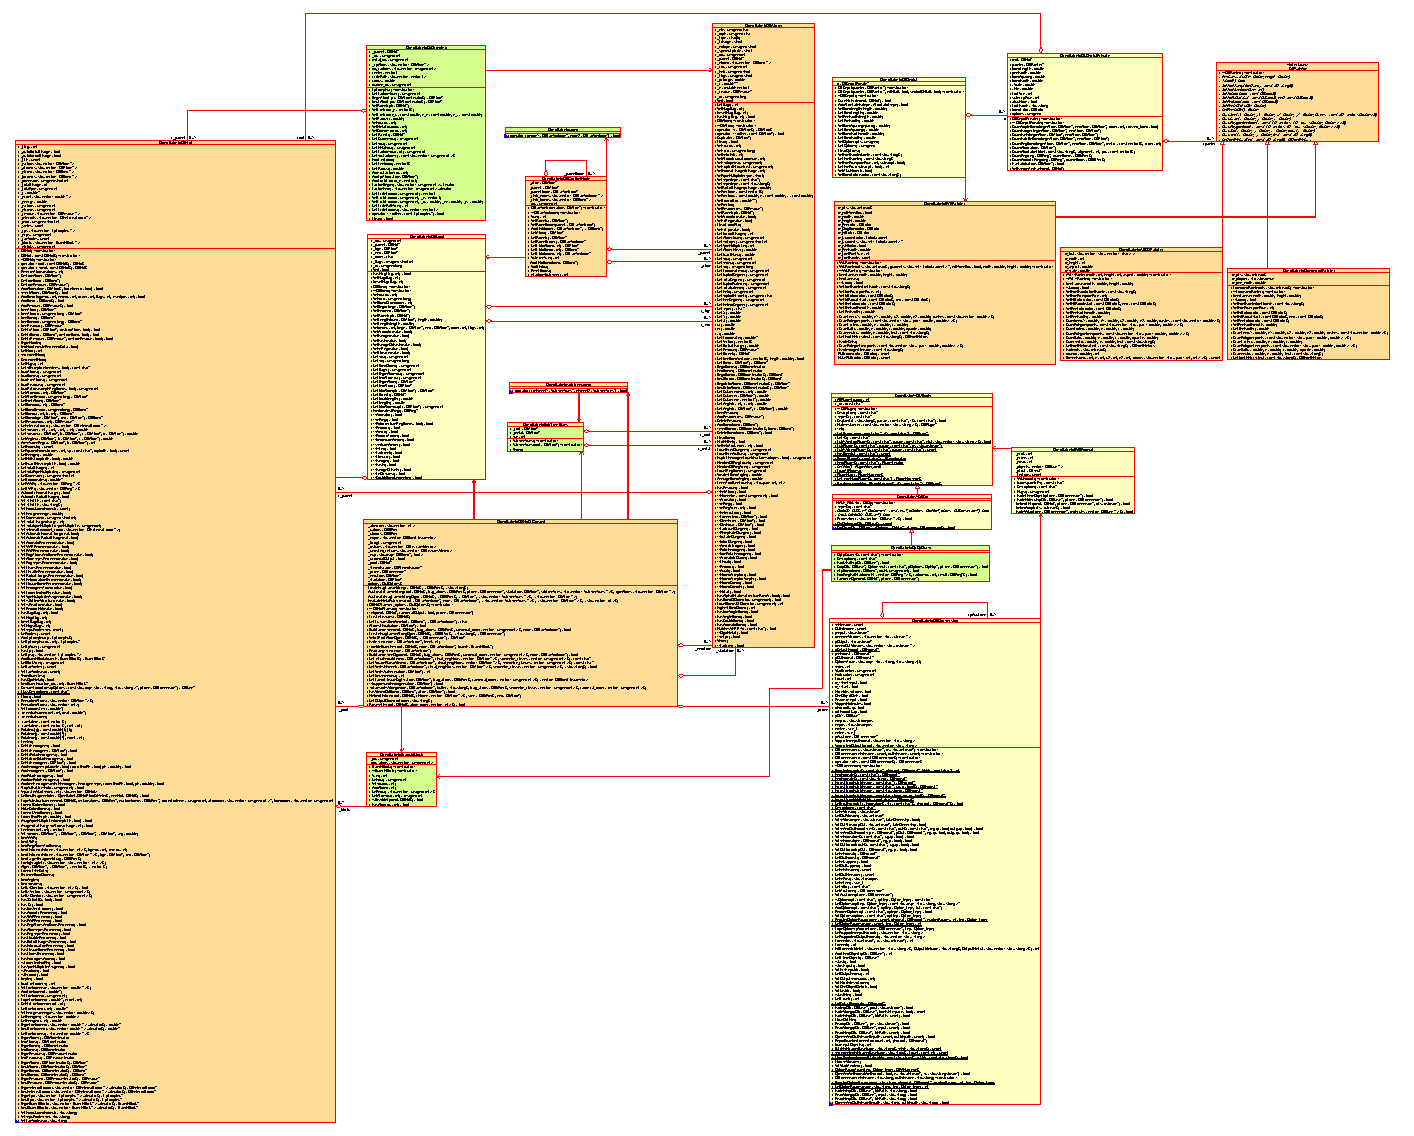
\includepdf[pages=-, offset=0 0,landscape=true,]{imagenes/diseno/diagramaClasesHorizontal_cropped.pdf}


Se pasa a detallar ahora cada una de ellas, tanto las modificadas como las nuevas, para qué sirven, y en qué consisten sus métodos brevemente. Las clases que no se han alterado, al igual que el resto de clases que no se incluyen en el diagrama se puede consultar su documentación en la página oficial \footnote{\url{https://openbabel.github.io/api/3.0/index.shtml}}. Puntualizar que existe una enorme cantidad de clases en la librería de OpenBabel, no tendería sentido añadirlas todas en el diagrama. Además, no todas poseen de documentación, por lo que la mayoría no aparecerán en la página anterior.

\section{Clases modificadas}
\begin{itemize}
    \item \textbf{OBPainter}: clase base abstracta para las clases de representación gráfica 2D. Se han añadido el siguiente método para poder utilizarlo en las clases que implementan esta interfaz:
    \begin{lstlisting}[language=C++]
        public: 
    
virtual void DrawPolygonLine(const std::vector<std::pair<double, double> >& points) = 0;
    \end{lstlisting}

    \item \textbf{SVGPainter}: clase que hereda de OBPainter y genera representaciones 2D en el formato de gráficos vectoriales SVG.
    \begin{lstlisting}[language=C++]
        public: 
    
//Inserts the necessary xml code in the .svg output file to draw a polygon according to the vector of points specified by @p points
void DrawPolygonLine(const std::vector<std::pair<double, double> >& points);
    \end{lstlisting}

    \item \textbf{ASCIIPainter}: clase que hereda de OBPainter.
    \begin{lstlisting}[language=C++]
        public: 
    
//The method is declared empty to avoid compilation errors due to interface implementation. It has no use 
void DrawPolygonLine(const std::vector<std::pair<double, double> >& points);
    \end{lstlisting}

    \item \textbf{CommandPainter}: clase que hereda de OBPainter.
    \begin{lstlisting}[language=C++]
        public: 
    
//The method is declared empty to avoid compilation errors due to interface implementation. It has no use 
void DrawPolygonLine(const std::vector<std::pair<double, double> >& points);
    \end{lstlisting}

    % -------------------------- Atom ---------------------------
    \item \textbf{OBAtom}: clase central, contiene la información relativa a un átomo. Se han añadido los siguientes métodos:
    \begin{lstlisting}[language=C++]
    public: 
    
//\return Is this a metal commonnly present in organometallic compounds?
bool IsOgmMetal();

//\return Is atom part of a Cp ring?
bool IsInCp() const;

//\return Is this atom a Carbon (atomic number == 6)?
bool IsCarbon();

//Debug method. Displays on basic output simple data to identify the atom
void Show();

//Mark an atom as part of a Cp ring
void SetInCp(bool value = true);
    \end{lstlisting}


    % -------------------------- Mol ---------------------------
    \item \textbf{OBMol}: clase central, almacena toda la información básica relacionada con una molécula. Se han añadido las siguientes variables y métodos:
    \begin{lstlisting}[language=C++]
    private: 
    
std::string _smiles;                //!< Input smiles string for the molecule
std::vector<CpComplex*> _cps;       //!< Cp information
unsigned int _ncps;                 //!< Number of cps complexes detected
std::string  _canSmiles;            //!< Canonical smiles based on Ogm canonicalization
std::vector<BranchBlock*> _blocks;  //!< Branches information
unsigned int _nblocks;              //!< Number of blocks


    public: 
    
//! Set the input smiles string of this molecule to @p smi
void SetInputSmiles(std::string smi);

//! \return the input smiles string of this molecule
std::string GetSmiles();

//! Add a new CpComplex specified by @p cp
void AddCpComplex(CpComplex& cp);

//! \return the cp at index @p idx or NULL if none exists.
CpComplex* GetCpComplex(int idx);

//! \return number of cp in the molecule
unsigned int GetCpSize();

//! \return whether the molecule has cps or not
bool HasCp();

//! \return the whole container of cps of this molecule
std::vector<CpComplex*> GetCps();

//! Add a new block to the molecule, specified by @p branch
BranchBlock* AddBranchBlock(BranchBlock& branch);

//! \return the number of blocks in the molecule
unsigned int GetBlockSize();

//! \return the canonical smiles string generated by the ogm canonicalization methods
std::string GetCanSmiles();

//! Set the canonical smiles string of this molecule to @p smi
void   SetCanSmiles(std::string smi);

//! Debug method. Displays on basic output all molecule blocks with basic information of the atoms.
void ShowBranches();

//! \return If this molecule has any Ogm metal or not
bool HasOgmMetal();

//! \return the block of which the carbon at index @p carbon_idx is part, or NULL if no such block exists
BranchBlock* FindBranch(int carbon_idx);

//! Set the iterator to the beginning of the Cp list
//! \return the first Cp structure, or NULL if none exist
CpComplex* BeginCp(std::vector<CpComplex*>::iterator & i);

//! Advance the iterator to the next Cp record
//! \return the next first Cp record, or NULL if none exist
CpComplex* NextCp(std::vector<CpComplex*>::iterator& i);

//! Set the iterator to the beginning of the BranchBlock list
//! \return the first BranchBlock structure, or NULL if none exist
BranchBlock* BeginBranchBlock(std::vector<BranchBlock*>::iterator& i);

//! Advance the iterator to the next BranchBlock record
//! \return the next first BranchBlock record, or NULL if none exist
BranchBlock* NextBranchBlock(std::vector<BranchBlock*>::iterator& i);
    \end{lstlisting}


    % -------------------------- OBMol2Cansmi ---------------------------
    \item \textbf{OBMol2Cansmi}: clase que maneja la conversión del smiles de entrada a un smiles canónico. Se han añadido los siguientes métodos:
    \begin{lstlisting}[language=C++]
        private: 
    
//Only changed visibility to private, since CreateFragCansmiStringOgm was created. Selects the "root" atom, which will be first in the SMILES, then builds a tree in canonical order, and finally generates the SMILES.
void CreateFragCansmiString(OBMol&, OBBitVec&, std::string&);

    
//Auxiliary private methods for SelectRootAtomOgm

//Shortened version of the CreateCansmiString method. Create the necessary variables to call AuxCreateFragCansmiStringOgm.
void AuxCreateCansmiString(OBMol& mol, OBBitVec& frag_atoms, OBConversion* pConv, OBAtom* startatom, std::vector<SubTreeSizes*>& subtreeSizes, std::vector<OBAtom*> ogmAtoms);

//Shortened version of the CreateFragCansmiStringOgm method. Create the necessary variables to build a new canonical tree using as root @p startAtom
void AuxCreateFragCansmiStringOgm(OBMol&, OBBitVec&, OBAtom*, std::vector<SubTreeSizes*>&, std::vector<OBAtom*>);

//Once the tree is built, this method runs through it in DFS evaluating the subtrees hanging from the other ogm metals. Use the auxiliary struct SubTreeSizes for this. 
void EvaluateMetalSubTrees(OBCanSmiNode* root, OBCanSmiNode* node, std::vector<SubTreeSizes*>&, std::vector<OBAtom*>&, std::vector<int>&);

        public: 
//Method based on CreateFragCansmiString. Share much of the code, with some additional methods specifically for my own canonical form designed for organometallic molecules.
void CreateFragCansmiStringOgm(OBMol&, OBBitVec&, std::string&, OBConversion*);

//If more than 1 Ogm metal is present in the molecule, this method chooses one of them, based on some rules and the conectivity of the metal within the molecule and the rest of the atoms
OBAtom* SelectRootAtomOgm(OBMol&, OBConversion*);

//Debug method for writing in basic output the tree with hierarchy formating
void WriteTree(OBCanSmiNode* node, int level = 0);

//Adds information to the molecule of the blocks that form it. Being a block, each set of atoms that, due to their bonds, are within the same parenthesis in the original input Smiles. Or, according to the OBMol2Cansmi::BuildCanonTree method, the parent-child relationship between atoms.
void IdentifyBranches(OBMol& mol,OBCanSmiNode* node, BranchBlock* branch = nullptr);

//Modifies the tree built by BuildCanonTree based on the length of the branches identified in IdentifyBranches. This is a canonical rule designed for a little more consistency in the output canon smiles.
void RearrangeTree(OBCanSmiNode* node);

//Builds the SMILES tree, in canonical order, for the specified molecular fragment. Based on the BuildCanonTree method. Shares much of the code, with some changes in the neighbour selection algorithm.
bool BuildCanonTreeOgm(OBMol& mol, OBBitVec& frag_atoms, vector<unsigned int>& canonical_order, OBCanSmiNode* node);
    \end{lstlisting}


    % -------------------------- OBCanSmiNode ---------------------------
    \item \textbf{OBCanSmiNode}: clase que representa un nodo. En conjunto se forma una estructura de árbol, cada nodo es un átomo del árbol para luego escribir el SMILES canónico. Se han añadido los elementos:
    \begin{lstlisting}[language=C++]
        private: 
    
OBCanSmiNode* _parentNode;      //!< Pointer to the parent node

//! Add a child bond to the node, specified by @p bond. Should only be used in the ResetBonds method as a part of the OBMol2Cansmi::RearrangeTree algorithm.
//! Otherwise, use addChildnode to add both the child node and its respective bonds
void AddChildBond(OBBond* bond);

        public: 

//! Set the parent node to @p parent
void SetParentNode(OBCanSmiNode* parent);

//! \return the parent node
OBCanSmiNode* GetParentNode();

//! Traverses the tree in dfs from the node calling the method
//! \return the number of total children (counting himself) 
int SubTreeSize();

//! Sort a node's child_nodes using a std::sort operation an a custom comparator 'mycomp'
void SortChilds();

//! When added at the same time in the addchildnode method, the child with its bond have a 1 to 1 index correspondence. When reordering the children, in OBMol2Cansmi::RearrangeTree, the indices of the bonds are lost. This method clears and adds the bonds back in order.
void ResetBonds();

//! \return the total number of carbons in this node subtree
int nCarbonsSubTree();
    \end{lstlisting}

\end{itemize}





\section{Clases nuevas}
\begin{itemize}
    % -------------------------- CpComplex ---------------------------
    \item \textbf{CpComplex}: clase que maneja y permite almacenar estructuras de ciclopentadienilo. Se han creado las siguientes variables y métodos:
    \begin{lstlisting}[language=C++]
	protected:
  
OBMol* _parent;                         //!< Parent molecule
unsigned int _idx;                      //!< Cp identifier within the molecule
unsigned int metal_idx;                 //!< Atom idx of central metal
std::vector<OBAtom*> _cpAtoms;          //!< Atoms for the carbons of the Cp structure
std::vector<unsigned int> idx_carbons;  //!< Atom indexes for the carbons of the Cp structure
vector3 center;                         //!< Cp center, for normal bond connection with metal atom, and aromatic circle position
std::vector<vector3> circlePath;        //!< Coordinates for the cp circle (needed to achieve a perspective circunference)
double radius;                          //!< Cp's aromatic circle radius
unsigned int dummy_idx;                 //!< Dummy central atom idx


        public:

//! Default constructor 
CpComplex();

//! \name Methods to modify internal information
//@{
//! Attach an OBMol @p ptr as the parent container for this Cp
void SetParent(OBMol* ptr);
//! Set the center point of the Cp, sprecified by @p _v. It is equidistant to every carbon in th Cp, as they are disposed in a regular polygon
void SetCentroid(vector3& _v);
//! Set the center point of the Cp, sprecified by @p v_x, v_y, v_z. It is equidistant to every carbon in th Cp, as they are disposed in a regular polygon
void SetCentroid(const double v_x, const double v_y, const double v_z);
//! Set the radius of the Cp circle
void SetRadius(double r);
//! Set the Cp identifier
void SetIdx(int idx);
//! Set the idx of the central metal to which this Cp is attached
void SetMetalIdx(int midx);
//! Dummy atom is created to make a perpendicular bond between the metal and the Cp drawing
//! Set the atom idx of the dummy atom created for this Cp 
void SetDummyIdx(int idx);
//! Set the point of the Cp circle at index @p i to the coordinates specified by @p _v
void SetCircleCoord(unsigned int i, vector3 _v);
//! Set the point of the Cp circle at index @p i to the coordinates specified by @p _vx, _vy, _vz
void SetCircleCoord(unsigned int i, double _vx, double _vy, double _vz = 0.0);
//@}


//! \name Methods to retrieve information
//@{
//! \return number of carbon atoms in the cp
unsigned int GetCarbonsSize();
//! \return the molecule which contains this Cp, or NULL if none exists
OBMol* GetParent();
//! \return dummy atom idx for this Cp structure, or 0 if none exists
unsigned int GetDummyIdx() const;
//! \return Cp identifier
unsigned int GetIdx() const;
//! \return Central metal identifier
unsigned int GetMetalIdx() const;
//! \return carbon idx at position @p i in tha container. Zero based access method to vector
unsigned int GetCarbonIdx(int i) const;
//! \return the whole contanier of carbon idx
const std::vector<unsigned int>& GetIdxCarbons();
//! \return the centroid of this Cp in a coordinate vector
vector3& GetCentroid();
//! \return the radius of the Cp circle
double GetRadius();
//! \return the coordinate vector for the Cp circle point at position @p i in the container. Zero based access method to vector
vector3 GetCircleCoord(unsigned int i);
//! \return the number of points of the Cp circle
int GetCirclePathSize() const;
//! \return the whole container of coordinates of the Cp circle
std::vector<vector3> GetCircleCoords() const;
//@}


//! \name Addition of data for a Cp
//@{
//! Adds a new atom idx to this Cp
void AddIdxCarbon(int idx);
//! Adds a new atom to this Cp
void AddCpAtom(OBAtom* atom);
//! Adds a new point to the coordinate vector that forms the Cp circle
void AddCircleCoord(vector3 _v);
//@}


//! \name Iteration methods
//@{
//! Set the iterator to the beginning of the Cp atom list
//! \return the first atom, or NULL if none exist
OBAtom* CpComplex::BeginAtomCp(OBAtomIterator& i);
//! Advance the iterator to the next atom in the Cp
//! \return the next first atom record, or NULL if none exist
OBAtom* CpComplex::NextAtomCp(OBAtomIterator& i);
//@}


//! \name Other operations
//@{
//! Calculate and set the centroid of this Cp, taking into consideration all atoms stored in _cpAtoms
void FindCentroid();
//! Equivalence operator
bool operator==(const CpComplex* other) const;
//@}




    \end{lstlisting}


    % -------------------------- BranchBlock ---------------------------
    \item \textbf{BranchBlock}: clase que representa un bloque definido dentro de la molécula, p.ej. un ciclo de benceno, un Cp, o toda una rama de un átomo. Se han añadido las siguientes variables y métodos:
    \begin{lstlisting}[language=C++]
        private: 
    
unsigned int _idx;                          //!< Block identifier
std::vector<unsigned int> vidx_atoms;       //!< Vector idx of the atoms that are part of the block.

        public: 

//! Default constructor
BranchBlock();

//! Destructor
~BranchBlock();

//! \return the size of the block (number of atoms in the block)
int Size();

//! \return the block identifier
unsigned int GetIdx();

//! Set the block identifier
void SetIdx(int idx);

//! Add an atom's idx to the block
void AddAtom(int i);

//! \return the idx of the atom at position @p i. Zero based access.
unsigned int GetAtomIdx(int i);

//! \return Whether the @p idx exists within the atoms already inserted in the block
bool HasAtom(int idx);

//! Cp will be possible if all the elements in the block are carbons up to that point and have a bond with an ogm metal.
//! \return whether or not it appears to be a Cp block
bool IsPossibleCp(OBMol &mol)
    \end{lstlisting}


    % -------------------------- OpCpDraw ---------------------------
    \item \textbf{OpCpDraw}: clase plugin que hereda de OBOp. Contiene el algoritmo de detección, identificación, y almacenamiento en la molécula de estructuras tipo Cp.
    \begin{lstlisting}[language=C++]

//! Default constructor
OpCpDraw(const char* ID);

//! Inherited method. 
//! Display through the output stream a brief description of the plugin.
const char* Description();

//! Inherited method. 
//! \return true if this op (plugin operation) is designed to work with the class of @p pOb, e.g. OBMol
virtual bool WorksWith(OBBase* pOb) const;

//! Inherited method. Required function that does the work. Normally return true, unless object is not to be output. 
virtual bool Do(OBBase* pOb, const char* OptionText = nullptr, OpMap* pOptions = nullptr, OBConversion* pConv = nullptr);

//! \return If @p bond is likely to be a cp-bond like
bool isCpBond(OBBond* bond, unsigned int idxM);

//! Finds the ring of which the carbon with idx @p carbonIdx is a part of, among the rings of @p rlist (obtained from a SSSR perspective), and stores it in @p result.
//! \returns whether it was found or not
bool FindRingWithCarbon(vector<OBRing*>& rlist, int carbonIdx, OBRing*& result);

//! Canonize the input SMILES and identify blocks
void CanonizeOgm(OBMol* mol, OBConversion* pConv); 
    \end{lstlisting}


    
    % -------------------------- SubTreeSizes ---------------------------
    \item \textbf{SubTreeSizes}: struct auxiliar creado para la selección del primer metal durante la canonización (se profundiza sobre esto en la sección \ref{reglas_canonizado}). Contiene las siguientes variables y métodos:
    \begin{lstlisting}[language=C++]

OBAtom* _root;      //!< Tree root
OBAtom* _metal;     //!< Metal to evaluate
int size;           //!< Size of the subtree for the _metal to evaluate

//! Default constructor
SubTreeSizes();

//! Parameter constructor. Creates a new object with _root as @p root
SubTreeSizes(OBAtom* root);

//! Debug method. Displays through basic output the struct information.
void Show();
    \end{lstlisting}


    % -------------------------- subtreecomp ---------------------------
    \item \textbf{subtreecomp}: objeto comparador que prioriza unos metales sobre otros en el proceso de selección del átomo raíz para el árbol (más en detalle en la Sección \ref{canonizacion}).
    \begin{lstlisting}[language=C++]
bool operator() (SubTreeSizes* element1, SubTreeSizes* element2) const;
    \end{lstlisting}


    % -------------------------- mycomp ---------------------------
    \item \textbf{mycomp}: objeto comparador que prioriza las ramas del árbol canónico durante el proceso de reordenación.
    \begin{lstlisting}[language=C++]
bool operator() (OBCanSmiNode* node1, OBCanSmiNode* node2);
    \end{lstlisting}


\end{itemize}




















